% !TEX root=frame_thesis.tex

\chapter{Details of the Model} \label{sec:APPpopgrowth}

\begin{figure}
	\centering
	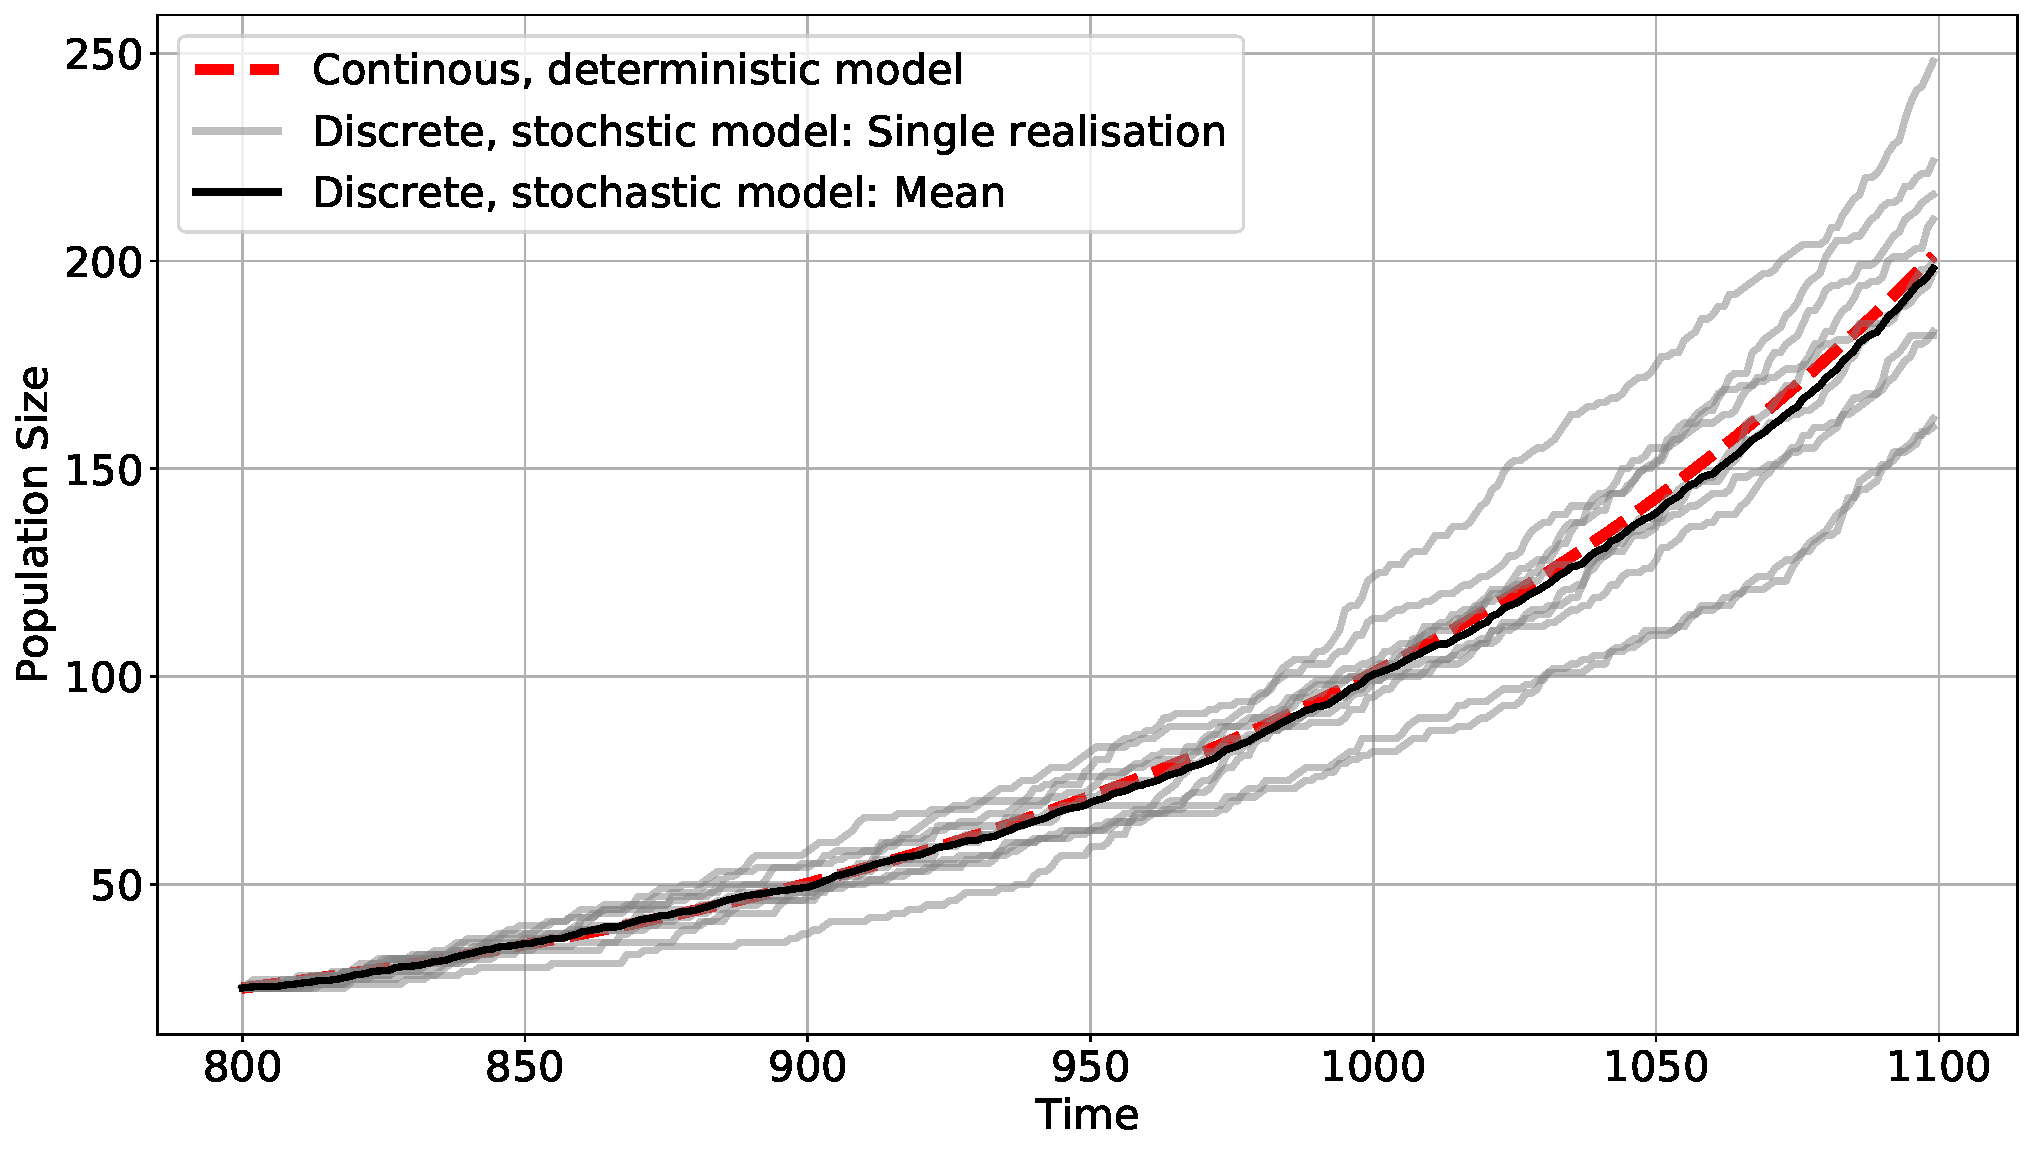
\includegraphics[width=\textwidth]{images/RealisationsOfPopGrowth.pdf}
	\caption{Realisations (and the mean) of the discrete, stochastic population growth model (assuming $H_{\rm i}(t) = 1$ for all $t$ here. In comparison, the continuous exponential growth. The growth rate is $g(H_{\rm i}(t)=1)=1.007$, as in the standard setting of the model.}
	\label{fig:realisationsofpopgrowth}
\end{figure}


\chapter{More results}
\section{Standard Run}
\begin{figure}
	\centering
	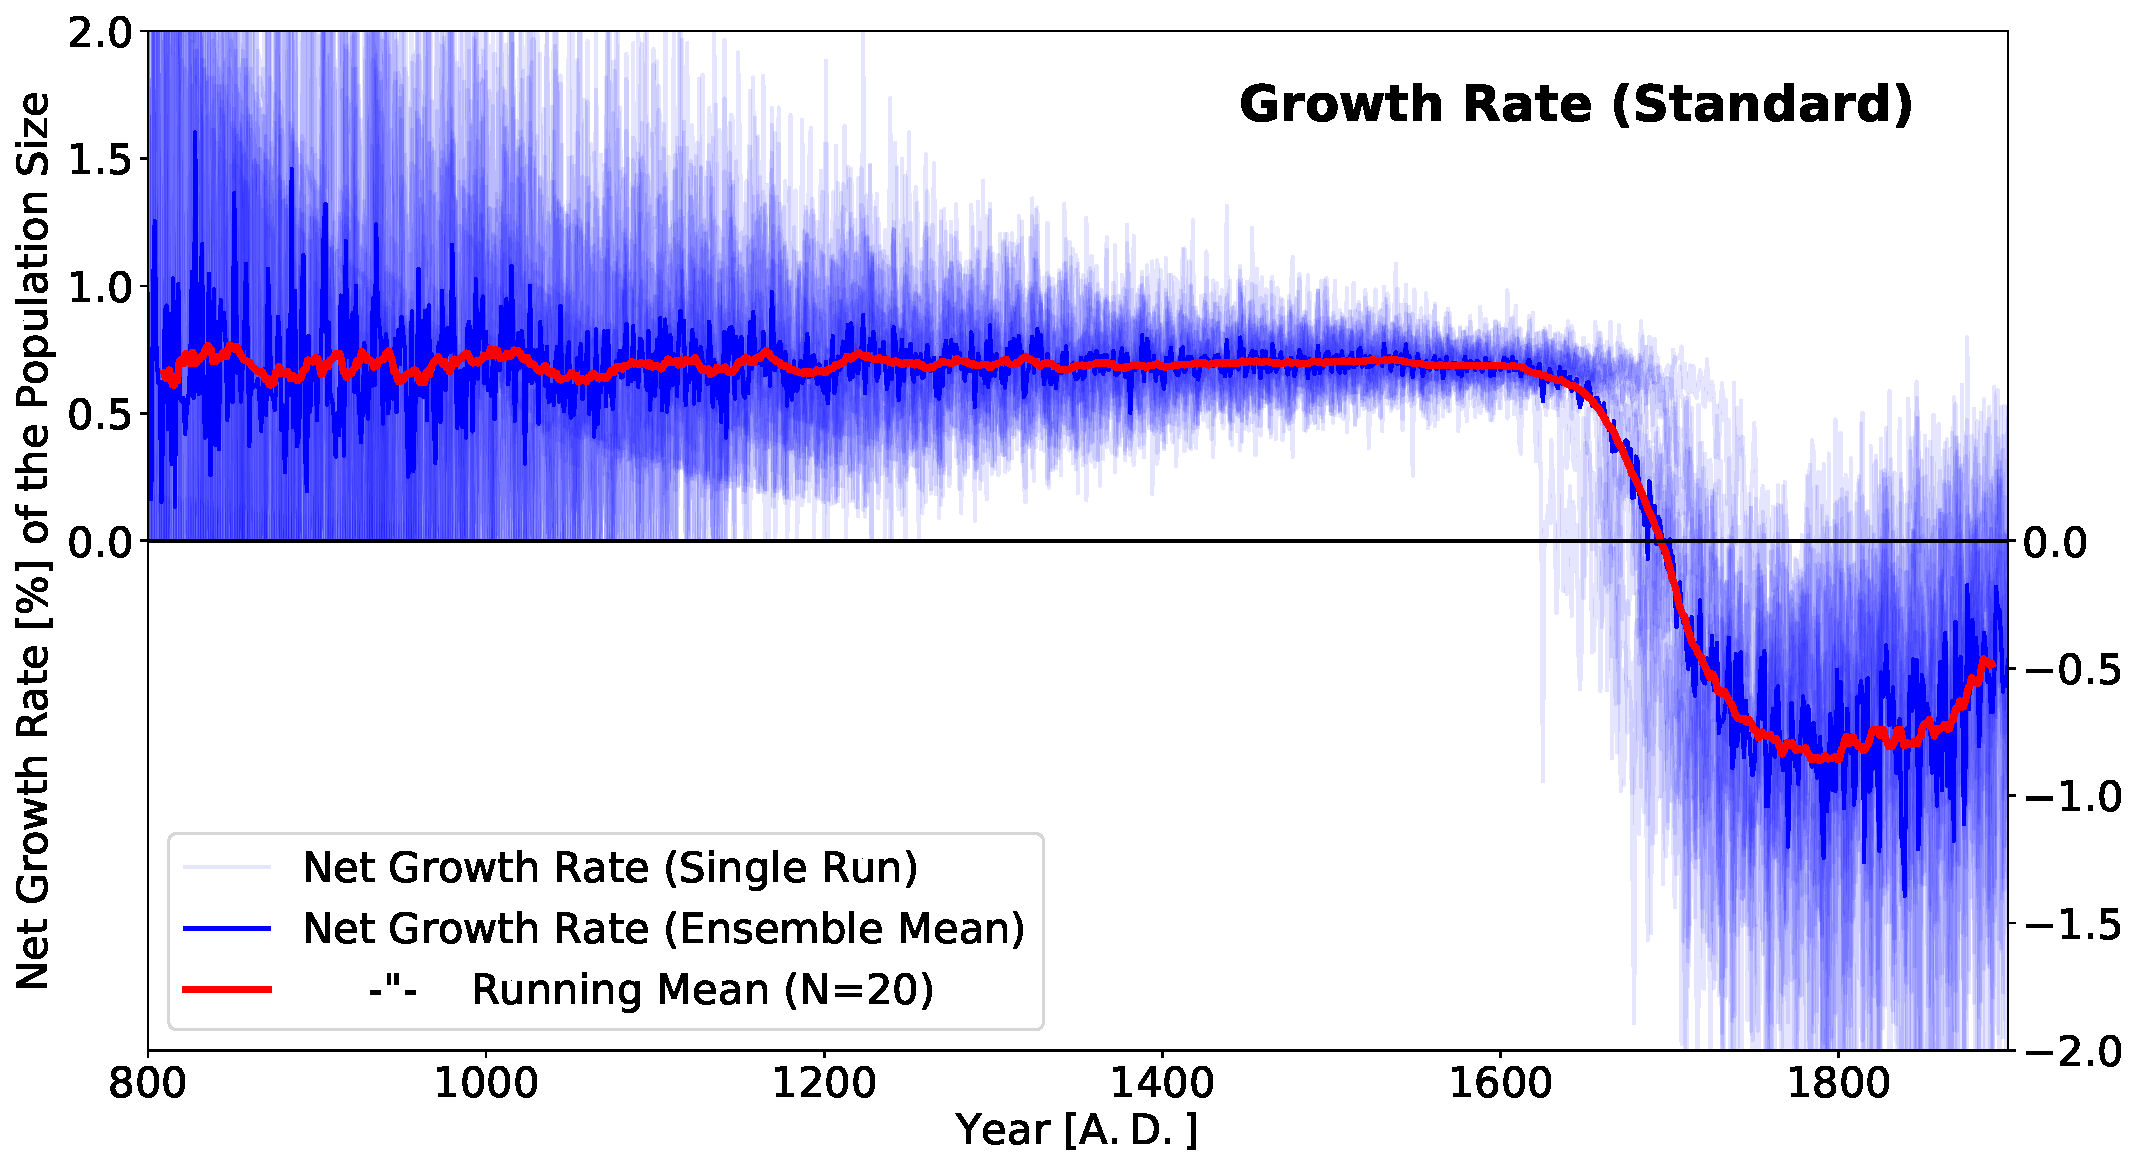
\includegraphics[width=1.0\linewidth]{images/Results/Standard/NetGrowthRate}
	\caption{Ensemble of five Standard runs. The net population growth rate is shown as the mean of the ensemble (blue) and, for easier visibility, as a running mean (red).} 
	\label{fig:app:STDnetgrowthrate}
\end{figure}
